\documentclass[letter, 12pt]{article}

\usepackage[margin=0.5in]{geometry}

%equation spacing
% \usepackage{xpatch}
\xapptocmd\normalsize{%
 \abovedisplayskip=0pt plus 0pt minus 0pt
 \abovedisplayshortskip=0pt plus 0pt
 \belowdisplayskip=0pt plus 0pt minus 0pt
 \belowdisplayshortskip=0pt plus 0pt minus 0pt
}{}{}

% \usepackage{blindtext}
\usepackage{amssymb,amsfonts,amsmath}

%%%%%%%%%%%%%%%%%%%%%%%%%%%%%%
%% OPTIONAL MACRO FILES
%% Insert self-defined macros here.
%% \newcommand definitions are recommended; \def definitions are supported

\usepackage[pdftex]{graphicx}
\usepackage{amsthm}
\usepackage{textcomp}
\usepackage{latexsym}
\usepackage{enumerate}
\usepackage{natbib}

\newtheorem{thm}{Theorem}[section]
\newtheorem{cor}[thm]{Corollary}
\newtheorem{ex}[thm]{Example}
\newtheorem{conj}[thm]{Conjecture}
\newtheorem{prob}[thm]{Problem}
\newtheorem{lem}[thm]{Lemma}
\newtheorem{prop}[thm]{Proposition}
\theoremstyle{definition}
\newtheorem{defn}[thm]{Definition}
\theoremstyle{remark}
\newtheorem{rem}[thm]{Remark}
%\numberwithin{equation}{section}

\newcommand{\set}[1]{\lbrace #1 \rbrace}
\newcommand{\setc}[2]{\lbrace #1 \mid #2 \rbrace}
\newcommand{\vv}[1]{{\mathbf{#1}}}
\newcommand{\dd}{{\mathrm{d}}}
\newcommand{\pd}[2]{\frac{\partial #1}{\partial #2}}
\newcommand{\pdn}[3]{\frac{\partial^#1 #2}{\partial #3^#1}}
\newcommand{\od}[2]{\frac{\dd #1}{\dd #2}}
\newcommand{\odn}[3]{\frac{\dd^#1 #2}{\dd #3^#1}}
\newcommand{\avg}[1]{\left< #1 \right>}

%--- operators
\DeclareMathOperator{\trop}{trop}
\DeclareMathOperator{\adj}{adj}
\DeclareMathOperator{\tr}{tr}
\DeclareMathOperator*{\argmax}{argmax}
\DeclareMathOperator{\Var}{Var}

\newcommand{\mb}{\mathbf}
\newcommand{\argmin}{\operatornamewithlimits{argmin}}
\newcommand{\doublebar}{\bigl|\!\bigr|}




\newcommand{\commentfe}[1]{{\color{red}FE: #1}}

\begin{document}

\title{Starter Manual for HDNET in Python}
\author{\normalsize Christopher Hillar, Redwood Center for Theoretical Neuroscience, Berkeley, CA 94720\\
\normalsize Felix Effenberger, Max-Planck-Institute for Mathematics in the Sciences, Leipzig, Germany
}
\date{}

\pagenumbering{gobble}


\maketitle



\textbf{Introduction}.  Here, we explore the basic functionality of the HDNET library in Python
\begin{center}
\texttt{https://github.com/qualiaphile/hdnet.git} \\
\end{center}

First we will make some fake spikes with correlated activity.  Let's initialize our script: \\

\texttt{import numpy as np}

\texttt{import matplotlib.pyplot as plt}

\texttt{from hdnet.spikes import Spikes}

\texttt{from hdnet.spikes\_\,model import SpikeModel, BernoulliHomogeneous, DichotomizedGaussian}  \\

We make two trials of 200 time points of spikes from $10$ neurons.   \\

\texttt{spikes\_\,arr = (np.random.random((2, 10, 200)) < .05).astype(int)}

\texttt{spikes\_\,arr[0, [1, 5], ::5] = 1 \# insert correlations}

\texttt{spikes\_\,arr[1, [2, 3, 6], ::11] = 1  \# insert correlations}

\texttt{spikes = Spikes(spikes\_\,arr=spikes\_\,arr)} \\

We can easily plot a raster of the trials and covariances: \\

\texttt{plt.matshow(spikes.rasterize(), cmap='gray')} 

\texttt{plt.title('Raw spikes')}

\texttt{plt.matshow(spikes.covariance().reshape((2 * 10, 10)), cmap='gray')}

\texttt{plt.title('Raw spikes covariance')}  \\

Next, we would like to model this noisy binary data.   First, we try to model each trial with a separate i.i.d. Bernoulli random binary vector having the same neuron means as in each trial:  \\

\texttt{spike\_\,model = BernoulliHomogeneous(spikes=spikes)}

\texttt{BH\_\,sample\_\,spikes = spike\_\,model.sample\_\,from\_\,model()}

\texttt{plt.matshow(BH\_\,sample\_\,spikes.rasterize(), cmap='gray')}

\texttt{plt.title('BernoulliHomogeneous sample')}

\texttt{plt.matshow(BH\_\,sample\_\,spikes.covariance().reshape((2 * 10, 10)), cmap='gray')}

\texttt{plt.title('BernoulliHomogeneous covariance')} \\

As we can see in Fig.~\ref{fake_ex_fig}, the samples from Bernoulli have the correct firing rates in each trial, but not the coordinated aspect (as can be seen in the covariance matrices for each trial, which are basically diagonal matrices).   A better model that keeps track of the correlations is the Dichotomized Gaussian \cite{bethge2008}: \\

\texttt{spike\_\,model = DichotomizedGaussian(spikes=spikes)}

\texttt{DG\_\,sample\_\,spikes = spike\_\,model.sample\_\,from\_\,model()}

\texttt{plt.matshow(DG\_\,sample\_\,spikes.rasterize(), cmap='gray')}

\texttt{plt.title('DichotomizedGaussian sample')}

\texttt{plt.matshow(DG\_\,sample\_\,spikes.covariance().reshape((2 * 10, 10)), cmap='gray')}

\texttt{plt.title('DichotomizedGaussian covariance')} \\


Finally, we try and model the data with a Hopfield network trained using MPF over all the trials:  \\

\texttt{spike\_\,model = SpikeModel(spikes=spikes)}

\texttt{spike\_\,model.fit()  \# note: this fits a single network to all trials}

\texttt{spike\_\,model.chomp()}

\texttt{converged\_\,spikes = Spikes(spikes\_\,arr=spike\_\,model.hopfield\_\,spikes\_\,arr)}

\texttt{plt.matshow(converged\_\,spikes.rasterize(), cmap='gray')}

\texttt{plt.title('Converge dynamics on Raw data')}

\texttt{plt.matshow(converged\_\,spikes.covariance().reshape((2 * 10, 10)), cmap='gray')}

\texttt{plt.title('Covariance of converged memories')} 	\\

 


\begin{figure}
\begin{center}
\textbf{a)}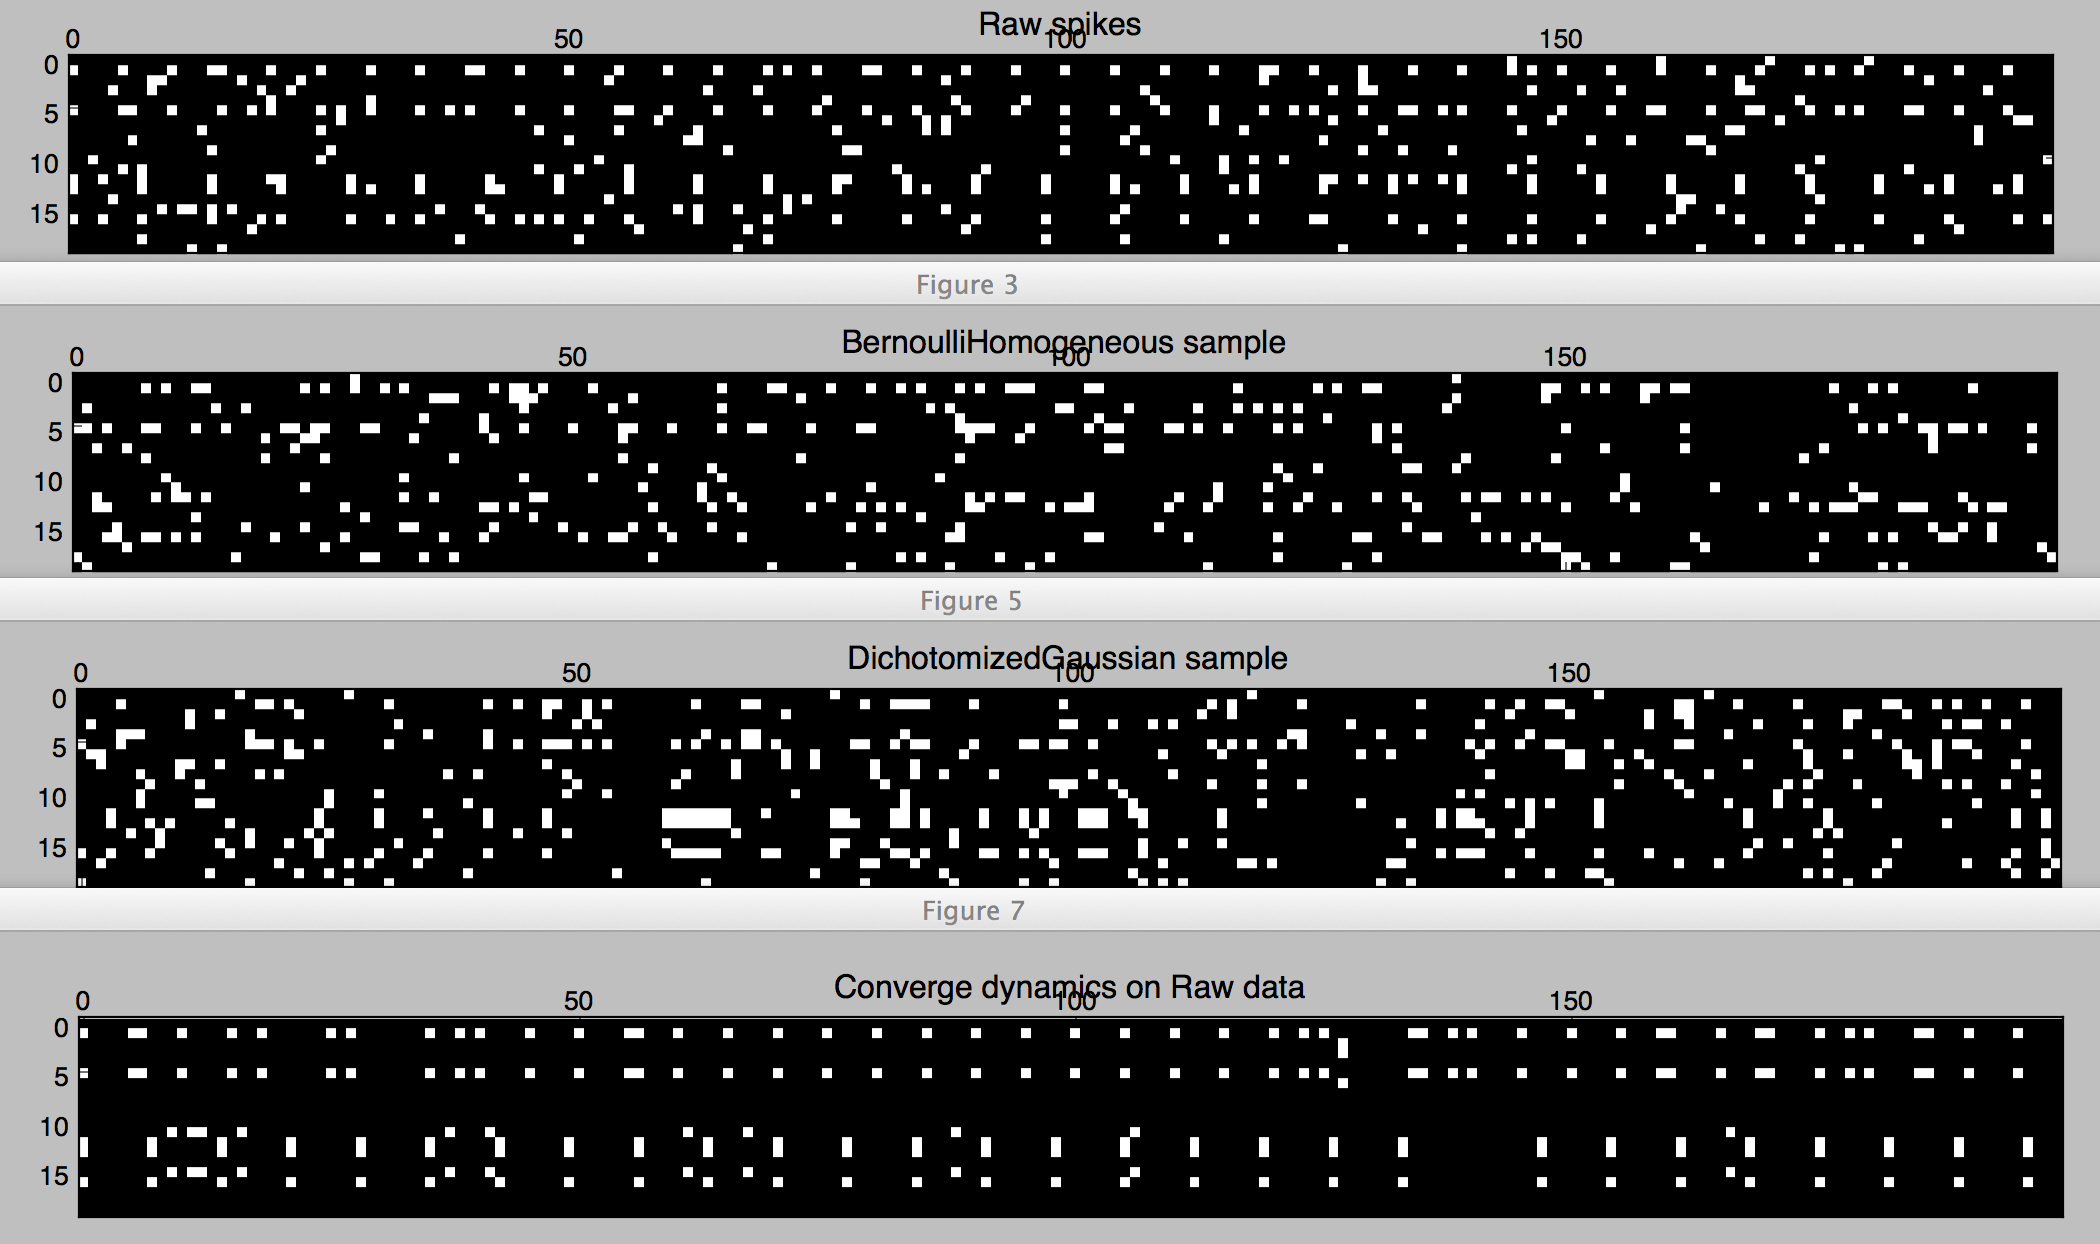
\includegraphics[width=.41\linewidth]{demo_fake_spikes.png} 
\textbf{b)}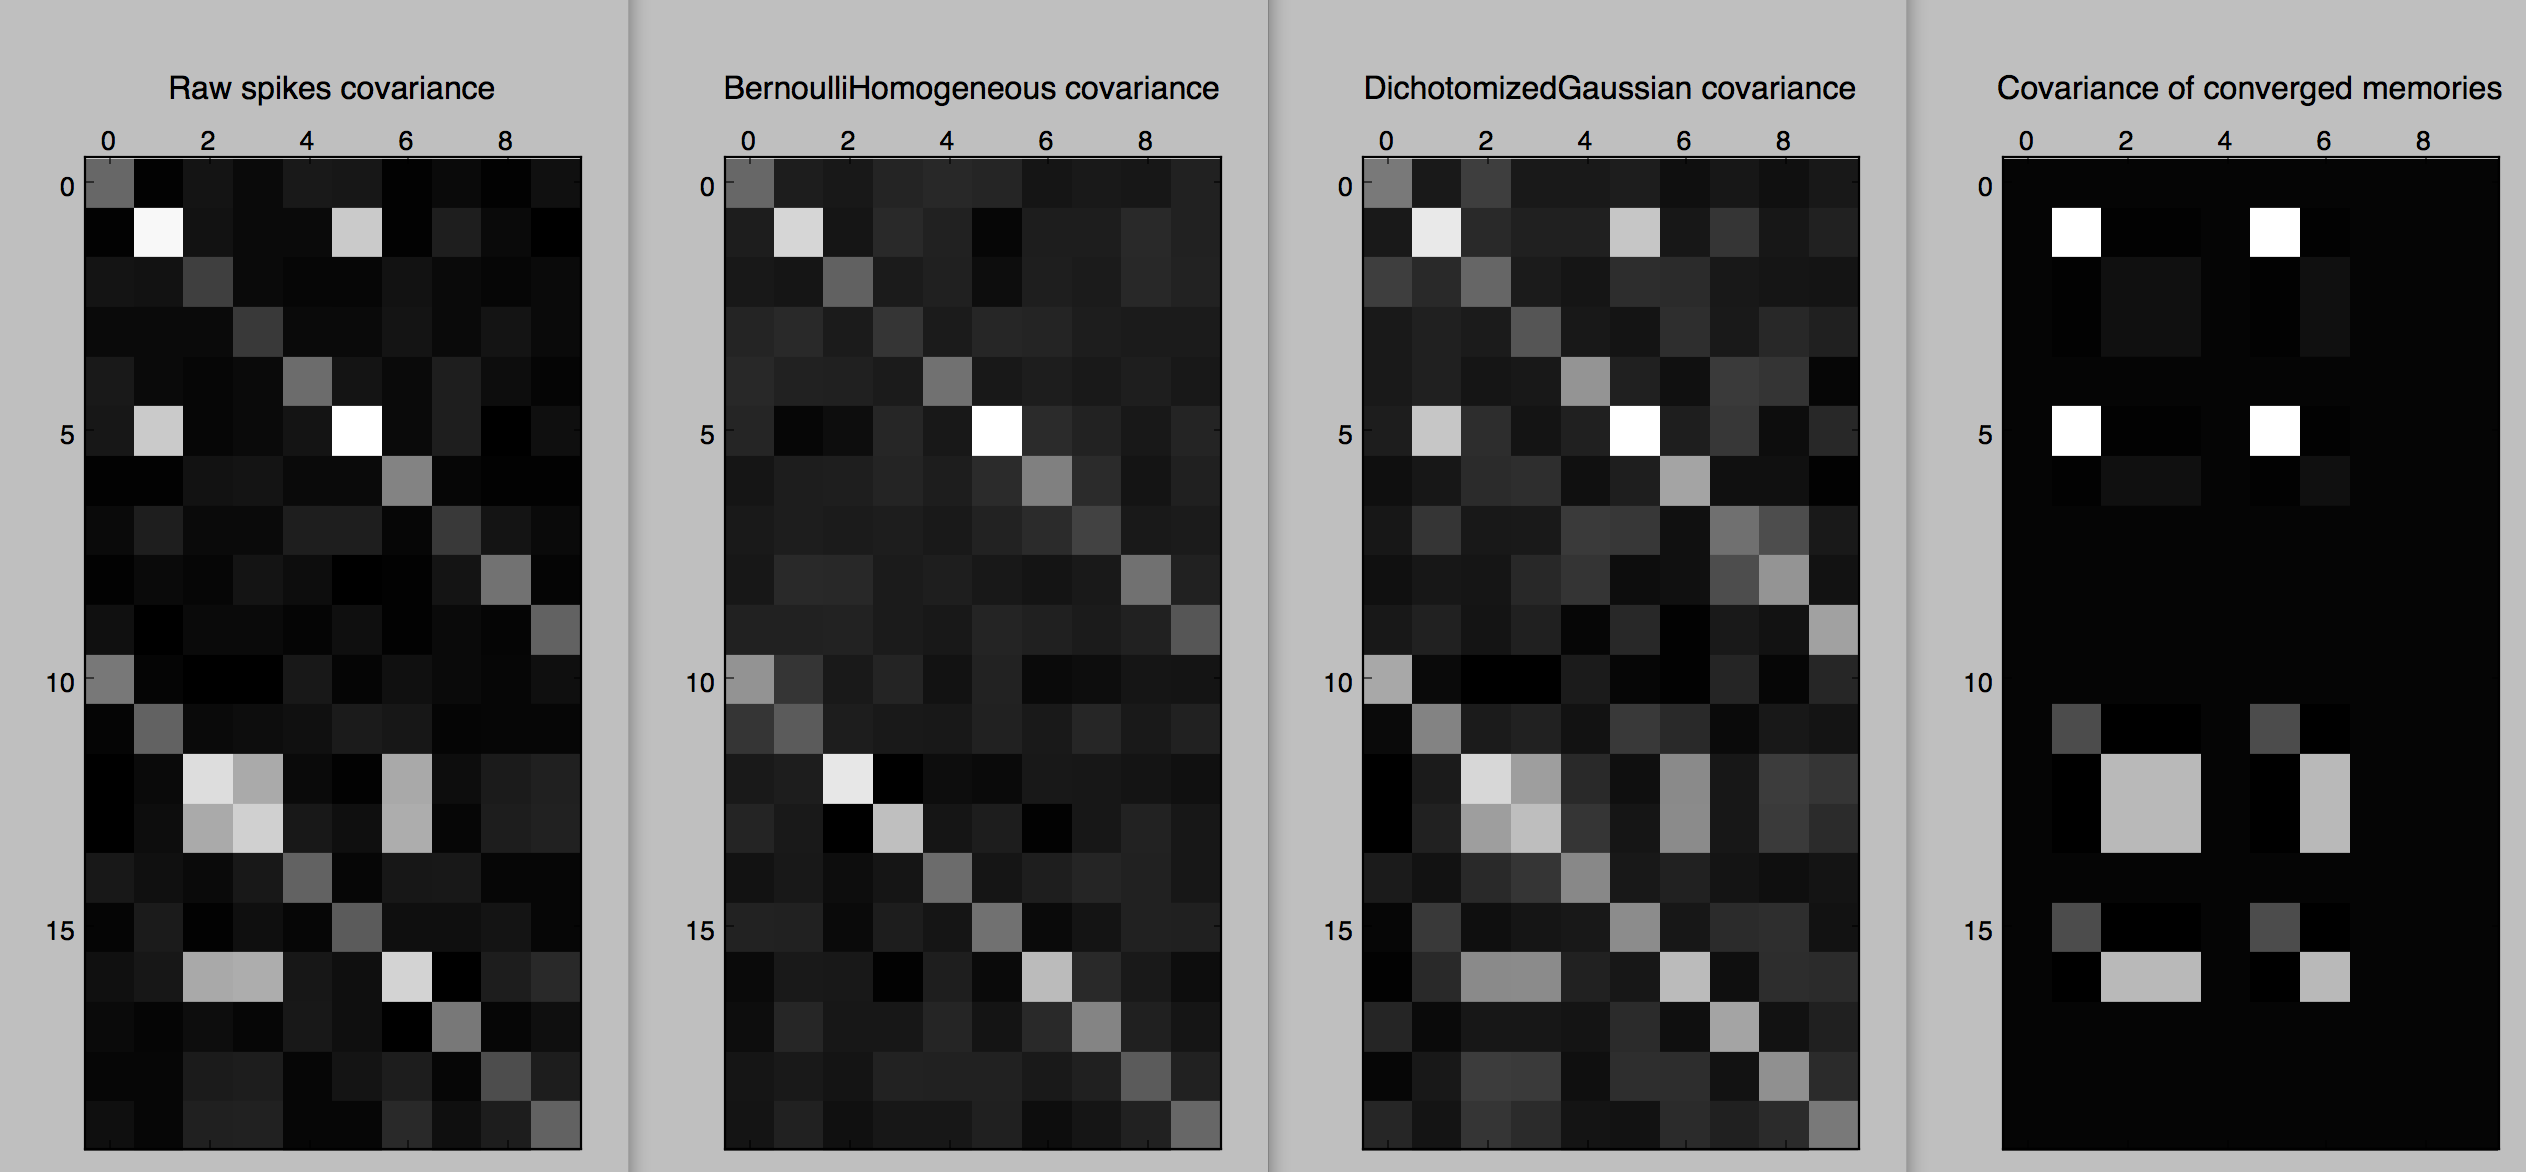
\includegraphics[width=.53\linewidth]{cov_demo.png} 
\caption{\textbf{Fake data example}. Two trials with 10 neurons.}
\label{fake_ex_fig}
\vspace{-.8cm}
\end{center}
\end{figure}



\textbf{More advanced features}.  One thing we would like to do is examine the structure of the memories: \\

\texttt{\# plot memory label (its chronological appearance) as a function of time}

\texttt{plt.figure()}

\texttt{plt.scatter(range(len(spike\_\,model.memories.sequence)),}

\texttt{\quad \quad \quad 1 + np.array(spike\_\,model.memories.sequence))}

\texttt{plt.xlabel('time bin')}

\texttt{plt.ylabel('Memory number (chronological order of appearance)')}

\texttt{plt.title('Converged memory label at each time bin')}

\texttt{\# versus the Raw data}

\texttt{plt.figure()}

\texttt{plt.scatter(range(len(spike\_\,model.emperical.sequence)),}

\texttt{\quad \quad \quad 1 + np.array(spike\_\,model.emperical.sequence))}

\texttt{plt.ylabel('Raw pattern number (chronological order of appearance)')}

\texttt{plt.xlabel('time bin')}

\texttt{plt.title('Raw pattern label at each time bin')}  \\
 
Notice in Fig.~\ref{fake_ex_fig2} that the converged dynamics of the trained Hopfield networks on the original data does reveal the 
hidden assemblies for the most part.

\begin{figure}[t!]
\begin{center}
\textbf{a)}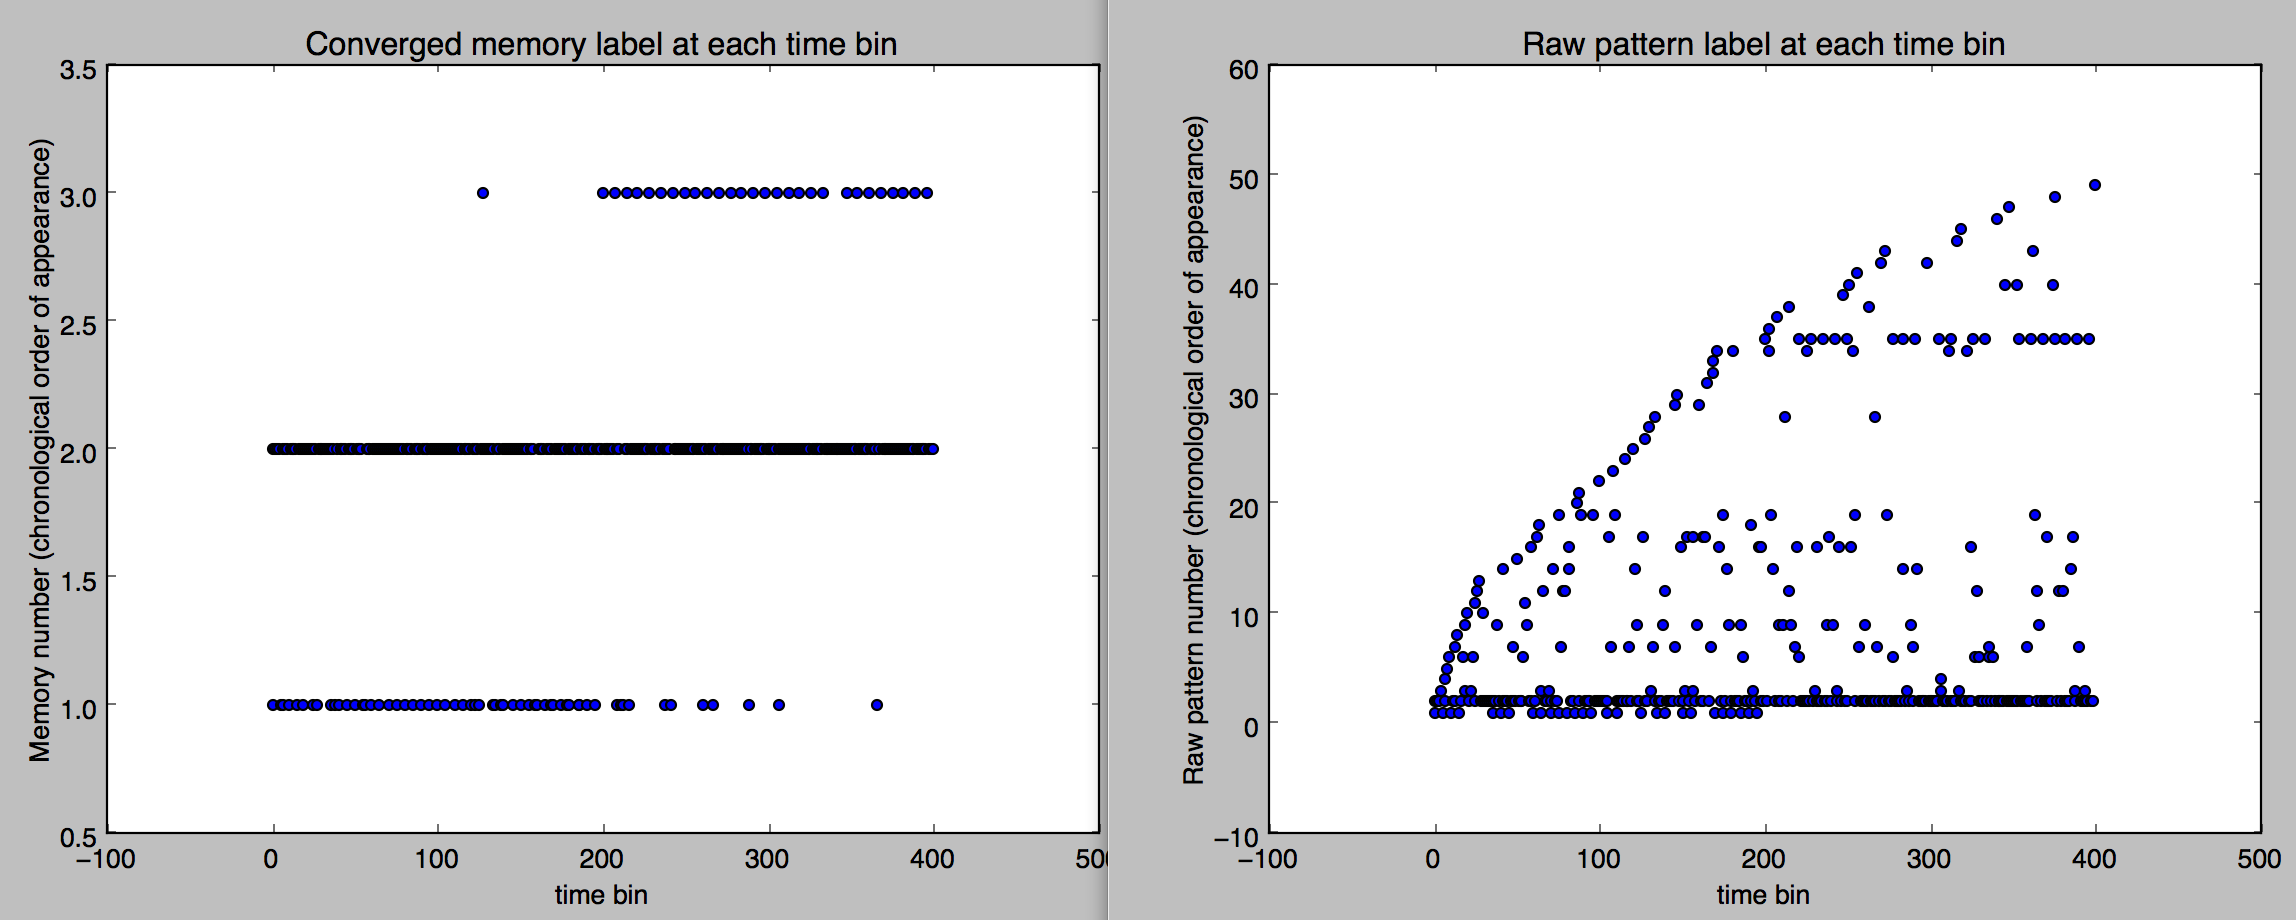
\includegraphics[width=.75\linewidth]{chron_order_patterns.png} 
%\textbf{b)}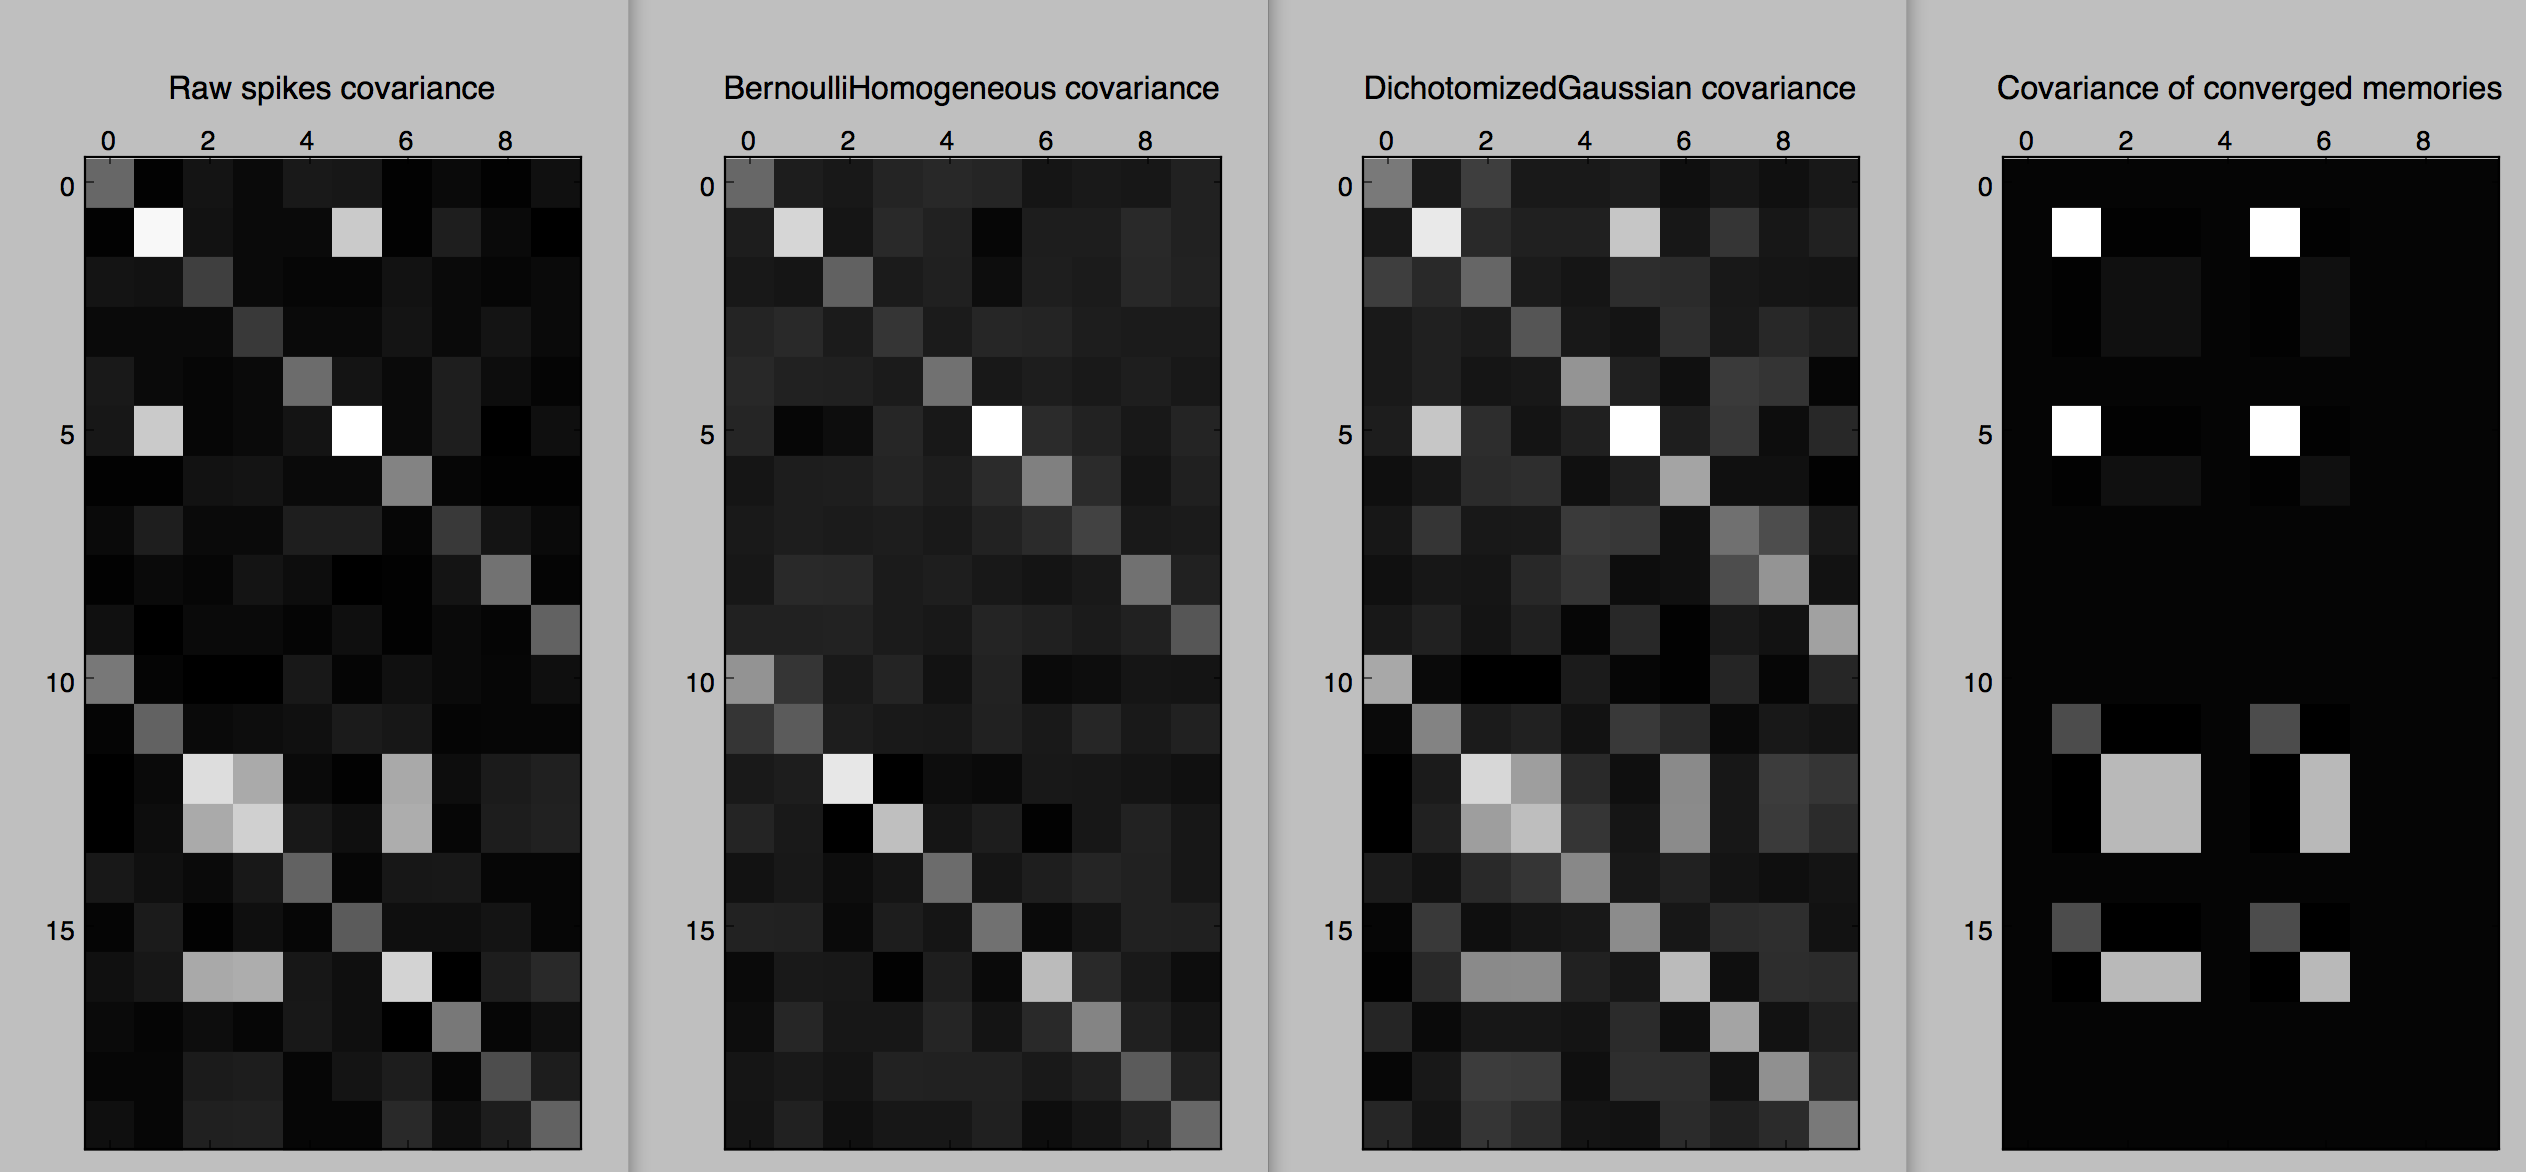
\includegraphics[width=.53\linewidth]{cov_demo.png} 
\textbf{b)}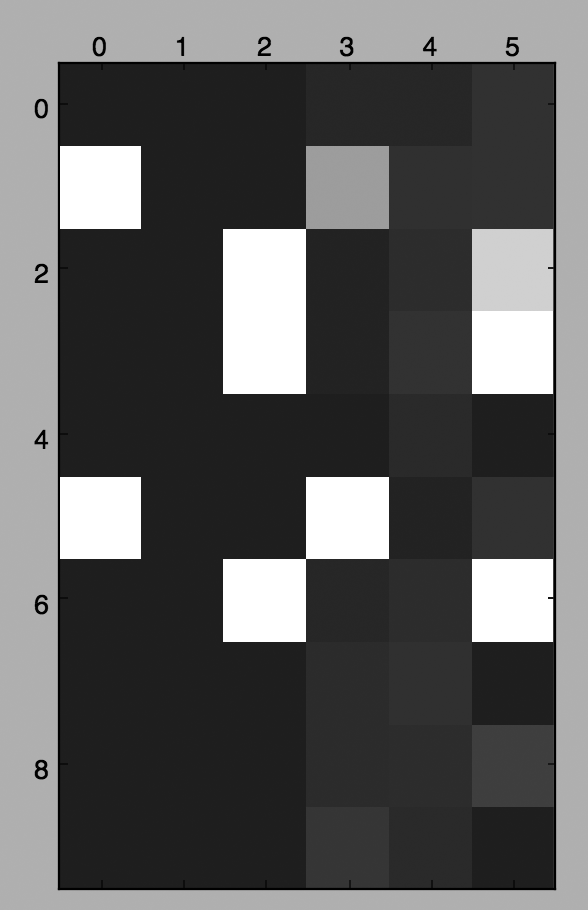
\includegraphics[width=.19\linewidth]{memories_stas.png} 
\caption{\textbf{Continuing fake data example}. \textbf{a)} Patterns (Converged at left, Raw on right) over time bins labeled on the $y$-axis by their first appearance in the dataset.  \textbf{b)}  Memories in network (left) and Memory Triggered Averages (at right).}
\label{fake_ex_fig2}
\vspace{-.8cm}
\end{center}
\end{figure}

Now that we know there are basically two assemblies, one showing up lots in the first trial and the other in the second.  Let's look at the
memories and their corresponding MTA's (\textit{memory triggered averages}).  The code below generates Fig.~\ref{fake_ex_fig2}\textbf{b}, which displays
a matrix whose first 3 columns are the memories in the network and whose next 3 columns are the average of Raw data patterns converging to the corresponding memory in the first 3 columns.  \\
 
\texttt{\# memories are ordered by their first appearance}
 
\texttt{bin\_\,memories = spike\_\,model.memories.fp\_\,list} 

\texttt{arr = np.zeros((spike\_\,model.original\_\,spikes.N, 2 * len(bin\_\,memories)))}

\texttt{for c, memory in enumerate(bin\_\,memories):}

\texttt{\quad \quad arr[:, c] = spike\_\,model.memories.fp\_\,to\_\,binary\_\,matrix(c)}

\texttt{for c, memory in enumerate(bin\_\,memories):}
 
\texttt{\quad \quad arr[:, c + len(bin\_\,memories)] = spike\_\,model.memories.stas[memory] /}

\texttt{\quad \quad \quad  spike\_\,model.memories.counts[memory]}

\texttt{print "Probabilities of each memory:"}

\texttt{print zip(bin\_\,memories, spike\_\,model.memories.to\_\,prob\_\,vect())} \\

\textbf{Saving}.  One can save Learners and Memories.



\scriptsize
\setlength{\bibsep}{0pt plus 0.3ex}
\bibliographystyle{abbrv}
\bibliography{hdnet_manual} 

\end{document}
